
This chapter presents the theoretical results bounding the error of
(piecewise) linear interpolation. The error analysis relies on linear
interpolation for three reasons: (1) second order results can be
obtained utilizing a Lipschitz constant on the gradient of a function,
rather than standard Lipschitz bounds; (2) the results directly apply
to Delaunay interpolation; and (3) multiple other interpolants in this
work compute predictions as convex combinations of observed function
values, which may allow for straight forward extensions of this error
bound.

\begin{lemma}
  \label{lemma:1}
  Let $S \subset \mathbb{R}^d$ be open and convex, $f: \mathbb{R}^d
  \rightarrow \mathbb{R}$, and $\nabla f \in
  Lip_{(\gamma,\|\cdot\|_2)}(S)$, the set of $\gamma$-Lipschitz
  continuous functions in the $2$-norm. Then for all $x,y \in S$
  $$\big|f(y) - f(x) - \langle \nabla f(x), y - x \rangle \big| \leq \frac{\gamma \|y - x\|_2^2}{2}.$$
\end{lemma}

\begin{proof}
  Consider the function $g(t) = f \big((1-t) x + t y \big)$, $0 \leq t
  \leq 1$, whose derivative $g'(t) = \big\langle \nabla f \big((1-t) x
  + t y \big), y - x \big\rangle$ is the directional derivative of $f$
  in the direction $(y - x).$
  \begin{align*}
    \big|f(y) - f(x) - \langle \nabla f(x), y - x \rangle \big|
       &= \big|g(1) - g(0) - g'(0) \big| & \\
       &= \bigg| \int_0^1 g'(t) - g'(0)\ dt \bigg| \\
       &\leq \int_0^1 \big|g'(t) - g'(0)\big|\ dt \\
       &= \int_0^1 \bigg| \big \langle \nabla f\big((1-t)x + ty\big) - \nabla f(x), y - x \big \rangle \bigg|\ dt \\
       &\leq \int_0^1 \big \| \nabla f\big((1-t)x + ty\big) - \nabla f(x) \big \|_2\ \| y - x \|_2\ dt \\
       &\leq \int_0^1 \big ( \gamma\ \|y-x\|_2 \big) \ \big( \|y-x\|_2 \big) t\ dt \\
       &= \frac{\gamma \|y - x\|_2^2}{2}.
  \end{align*}
\end{proof}

\begin{lemma}
  \label{lemma:2}
  Let $x, y, v_i \in \mathbb{R}^d$, $c_i \in \mathbb{R}$, and
  $|\langle y - x, v_i \rangle| \leq c_i$ for $i = 1$, $\ldots$, $d.$
  If $M = (v_1$, $\ldots$, $v_d)$ is nonsingular, then
  $$\|y - x\|_2^2 \leq \frac{1}{\sigma_d^2} \sum_{i=1}^d c_i^2,$$
  where $\sigma_d$ is the smallest singular value of $M.$
\end{lemma}

\begin{proof}
  Using the facts that $M$ and $M^t$ have the same singular values,
  and $\|M^tw\|_2 \geq \sigma_d \|w\|_2$, gives
  \begin{align*}
    \|y - x\|_2^2 &\leq \frac{\|M^t (y - x)\|_2^2}{\sigma_d^2} \\
                  &=    \frac{1}{\sigma_d^2} \sum_{i=1}^d \langle y - x, v_i \rangle^2 \\
                  &\leq \frac{1}{\sigma_d^2} \sum_{i=1}^d c_i^2.
  \end{align*}
\end{proof}

\begin{lemma}
  \label{lemma:3}
  Given $f$, $\gamma$, $S$ as in {\it Lemma \ref{lemma:1}}, let $X =
  \{x_0$, $x_1$, $\ldots$, $x_d\}$ $\subset S$ be the vertices of a
  $d$-simplex, and let $\hat f(x) = \langle c, x - x_0 \rangle +
  f(x_0)$, $c \in \mathbb{R}^d$ be the linear function interpolating
  $f$ on $X.$ Let $\sigma_d$ be the smallest singular value of the
  matrix $M = (x_1 - x_0$, $\ldots$, $x_d - x_0)$, and $k =
  \max\limits_{1\ \leq\ j\ \leq\ d} \|x_j - x_0\|_2.$ Then
  $$\big\|\nabla f(x_0) - c\big\|_2 \leq \sqrt{d} \frac{\gamma k^2}{\sigma_d}.$$
\end{lemma}

\begin{proof}
  Consider $f(x) - \hat f(x)$ along the line segment $z(t) = (1-t)x_0
  + t x_j$, $0 \leq t \leq 1.$ By Rolle's Theorem, for some $0 < \hat
  t < 1$, $\big\langle \nabla f\big(z(\ \hat t\ )\big) - c, x_j - x_0
  \big\rangle = 0.$ Now
  \begin{align*}
    \big| \big< \nabla f(x_0) - c, x_j - x_0 \big \rangle \big|
        &= \big| \big< \nabla f(x_0) - \nabla f\big(z(\ \hat t\ )\big) + \nabla f\big(z(\ \hat t\ )\big) - c, x_j - x_0 \big \rangle \big| \\
	&= \big| \big\langle \nabla f(x_0) - \nabla f \big(z(\ \hat t\ )\big), x_j - x_0 \big \rangle \big| \\
	&\leq \big \| \nabla f(x_0) - \nabla f\big(z(\ \hat t\ )\big) \big \|_2 \|x_j - x_0\|_2 \\
	&\leq \gamma \|x_0 - z(\ \hat t\ )\|_2\ \|x_j - x_0\|_2 \\
	&\leq \gamma \|x_j - x_0\|_2^2 \leq \gamma k^2, \\
  \end{align*}
  for all $1 \leq j \leq d.$ Using {\it Lemma \ref{lemma:2}},
  $$\big \| \nabla f(x_i) - c \big \|_2^2 \leq \frac{d}{\sigma_d^2}
  \big( \gamma k^2\big)^2 \implies \big \| \nabla f(x_i) - c \big \|_2
  \leq \sqrt{d} \frac{\gamma k^2}{\sigma_d}.$$
\end{proof}

\begin{theorem}
  Under the assumptions of {\it Lemma \ref{lemma:1}} and {\it Lemma
    \ref{lemma:3}}, for $z \in S$,
  $$ \big|f(z) - \hat f(z)\big| \leq \frac{\gamma \|z - x_0\|_2^2}{2} + \sqrt{d} \frac{\gamma k^2}{\sigma_d} \|z - x_0\|_2.$$
\end{theorem}

\begin{proof}
  Let $v = \nabla f(x_0) - c$, where $\|v\|_2 \leq \sqrt{d} \gamma k^2 / \sigma_d$ by {\it Lemma \ref{lemma:3}}. Now
  \begin{align*}
    \big|f(z) - \hat f(z)\big|
       &= \big|f(z) - f(x_0) - \langle c, z - x_0 \rangle \big| \\ 
       &= \big|f(z) - f(x_0) - \langle \nabla f(x_0) - v, z - x_0 \rangle \big| \\
       &= \big|f(z) - f(x_0) - \langle \nabla f(x_0) , z - x_0 \rangle + \langle v , z - x_0 \rangle \big| \\
       &\leq \big|f(z) - f(x_0) - \langle \nabla f(x_0) , z - x_0 \rangle \big| + \big| \langle v , z - x_0 \rangle \big| \\
       &\leq \big|f(z) - f(x_0) - \langle \nabla f(x_0) , z - x_0 \rangle \big| + \|v\|_2 \|z - x_0\|_2 \\
       &\leq \big|f(z) - f(x_0) - \langle \nabla f(x_0), z - x_0 \rangle \big| + \textstyle{\frac{\gamma k^2 \sqrt{d}}{\sigma_d}} \|z - x_0\|_2 \\
       &\leq \frac{\gamma \|z - x_0\|_2^2}{2} + \sqrt{d}\frac{\gamma k^2}{\sigma_d} \|z - x_0\|_2,
  \end{align*}
  where the last inequality follows from {\it Lemma \ref{lemma:1}}.
\end{proof}


In summary, the approximation error of a linear (simplicial)
interpolant tends quadratically towards zero when approaching observed
data only when the diameter of the simplex is also reduced at a
proportional rate.  Only linear convergence to the true function can
be achieved in practice, without the incorporation of additional
observations. Notice that the approximation error is largely
determined by the spacing of observed data. Predictions made by
simplices whose vertices are not well-spaced (i.e., have large
diameter, or are nearly contained in a hyperplane) have higher
error. In light of this error bound, an empirical evaluation of
presented algorithms follows.

%% ===================================================================
\vspace{-2mm}
\section{Data and Empirical Analysis}
\label{sec:error_data}

The theoretical results constructed at the start of this chapter for
(piecewise) linear interpolation are promising and apply directly to
Delaunay interpolation, however they are difficult to interpret in
context with approximation algorithms that do not have similar known
uniform error bounds. For that reason, this chapter utilizes five
different data sets of varying dimension and application to construct
approximations and compare the accuracy of different techniques.

In the following five subsections the sources and targets of each test
data set are described, as well as challenges and limitations related
to approximating these data. The distribution of response values being
modeled is presented followed by the distribution of approximation
errors for each algorithm. The plots for all five data sets have the
same format.

All five data sets are rescaled such that the domain of approximation
is the unit hypercube. The range of the first four data sets is the
real numbers, while the range of the fifth data set is the space of
cumulative distribution functions. All approximation techniques are
applied to the first four data sets, while only those interpolants
whose approximations are convex combinations of observed data are
applied to the final data set.

All approximations are constructed using $k$-fold cross validation as
described in \cite{kohavi1995study} with $k=10$. This approach
randomly partitions data into $k$ (nearly) equal sized sets. Each
algorithm is then evaluated by constructing an approximation over each
unique union of $k-1$ elements of the partition, making predictions
for points in the remaining element. As a result, each observed data
point is used in the construction of $k-1$ different approximations
and is approximated exactly once. The $k$-fold cross validation method
is data-efficient and provides an unbiased estimate of the expected
prediction error \cite{kohavi1995study}, however it should be noted
that neither this method nor others can provide a universally unbiased
estimator for the variance of prediction error \cite{bengio2004no}.

In addition to the figures displaying approximation results for each
data set, tables of accompanying numerical results are located in the
Appendix. All of the test data sets capture underlying functions that
are almost certainly stochastic. As described in Section
\ref{sec:introduction}, regression techniques appear most appropriate
for these problems. However, typically data grows exponentially more
sparse with increasing dimension. Given sparse data, regressors tend
towards interpolation.

%% -------------------------------------------------------------------
\subsection{Forest Fire ($n = 504$, $d = 12$)}

\begin{figure}
  \centering
  \begin{tikzpicture}
    \node (img)  {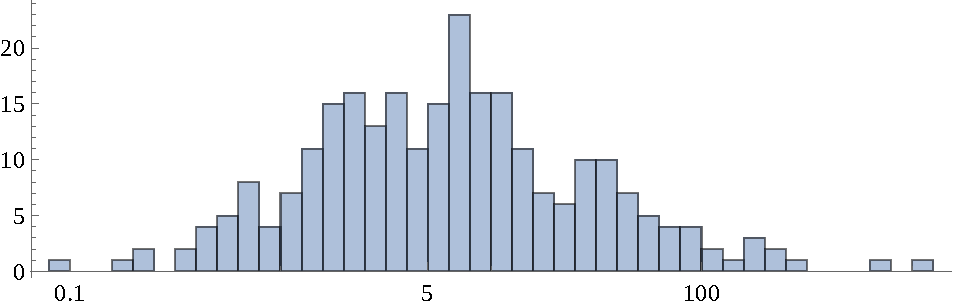
\includegraphics[width=0.75\textwidth,]{Figures/NA/Fig2.pdf}};
    \node[below=of img, node distance=1cm, yshift=1cm] {Forest Fire Area Burned};
    \node[left=of img, node distance=0cm, rotate=90, anchor=center,yshift=-0.7cm] {Count};
  \end{tikzpicture}
  \caption{Histogram of forest fire area burned under recorded weather
    conditions. The data is presented on a $\ln$ scale because
    most values are small with exponentially fewer fires on record
    that burn large areas.}
  \label{fig:hist-forest-fire}
\end{figure}

\begin{figure}
  \centering
  \begin{tikzpicture}
    \node (img)  {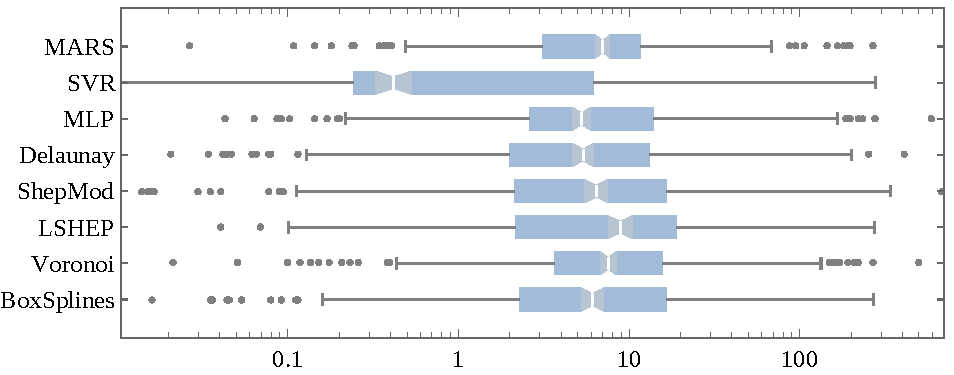
\includegraphics[width=0.8\textwidth,]{Figures/NA/Fig3.pdf}};
    \node[below=of img, node distance=1cm, yshift=1cm] {Area Burned Error};
  \end{tikzpicture}
  \caption{All models are applied to approximate the amount of area
    that would be burned given environment conditions. $10$-fold cross
    validation as described in the beginning of Section \ref{sec:error_data}
    is used to evaluated each algorithm. This results in exactly one
    prediction from each algorithm for each data point. These boxes
    depict the median (middle bar), median $95\%$ confidence interval
    (cones), quartiles (box edges), fences at $3/2$ interquartile
    range (whiskers), and outliers (dots) of absolute prediction error
    for each model. Similar to Figure \ref{fig:hist-forest-fire}, the
    errors are presented on a $\ln$ scale. The numerical data
    corresponding to this figure is provided in Table
    \ref{table:error-forest-fire} in the Appendix.}
  \label{fig:error-forest-fire}
\end{figure}


The forest fire data set \cite{cortez2007data} describes the area of
Montesinho park burned over months of the year along with
environmental conditions. The twelve dimensions being used to model
burn area are the $x$ and $y$ spatial coordinates of burns in the
park, month of year (mapped to $x$, $y$ coordinates on a unit circle),
the FFMC, DMC, DC, and ISI indices (see source for details), the
temperature, relative humidity, wind speed, and outdoor rain. The
original analysis of this data set demonstrated it to be difficult to
model, likely due to the skew in response values.

As suggested by Figure \ref{fig:error-forest-fire}, the SVR has the
lowest absolute prediction errors for $80\%$ of the data, with MLP and
Delaunay being the nearest overall competitors. The effectiveness of
SVR on this data suggests the underlying function can be defined by
relatively few parameters, as well as the importance of capturing the
low-burn-area data points.
%% -------------------------------------------------------------------



%% -------------------------------------------------------------------
\subsection{Parkinson's Telemonitoring ($n = 5875$, $d = 19$)}

\begin{figure}
  \centering
  \begin{tikzpicture}
    \node (img)  {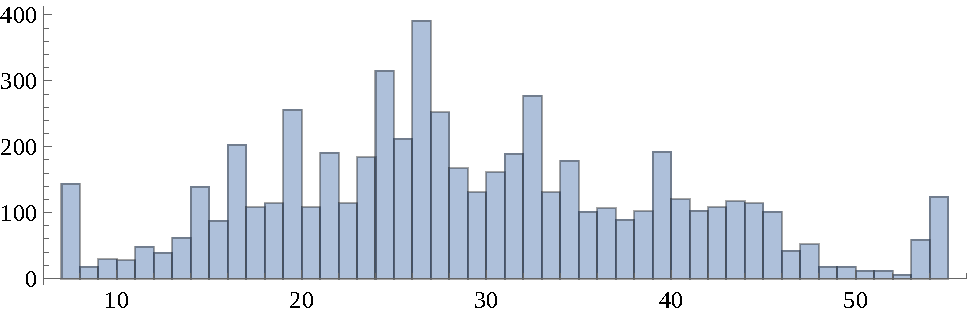
\includegraphics[width=0.75\textwidth,]{Figures/NA/Fig4.pdf}};
    \node[below=of img, node distance=1cm, yshift=1cm] {Parkinson's Total UPDRS Score};
    \node[left=of img, node distance=0cm, rotate=90, anchor=center,yshift=-0.7cm] {Count};
  \end{tikzpicture}
  \caption{Histogram of the Parkinson's patient total UPDRS clinical
    scores that will be approximated by each algorithm.}
  \label{fig:hist-parkinsons}
\end{figure}

\begin{figure}
  \centering
  \begin{tikzpicture}
    \node (img)  {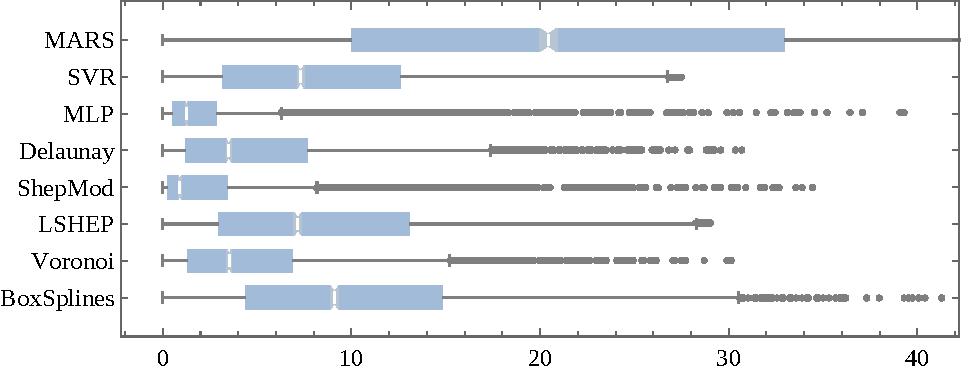
\includegraphics[width=0.8\textwidth,]{Figures/NA/Fig5.pdf}};
    \node[below=of img, node distance=1cm, yshift=1cm] {Total UPDRS Score Error};
  \end{tikzpicture}
  \caption{All models are applied to approximate the total UPDRS score
    given audio features from patients' home life, using $10$-fold
    cross validation. These boxes depict the median (middle bar),
    median $95\%$ confidence interval (cones), quartiles (box edges),
    fences at $3/2$ interquartile range (whiskers), and outliers
    (dots) of absolute prediction error for each model. The numerical
    data corresponding to this figure is provided in Table
    \ref{table:error-parkinsons} in the Appendix.}
  \label{fig:error-parkinsons}
\end{figure}

The second data set for evaluation \cite{tsanas2010accurate} is
derived from a speech monitoring study with the intent to
automatically estimate Parkinson's disease symptom development in
Parkinson's patients. The function to be approximated is a
time-consuming clinical evaluation measure referred to as the UPDRS
score. The total UPDRS score given by a clinical evaluation is
estimated through 19 real numbers generated from biomedical voice
measures of in-home sound recordings.

Figure \ref{fig:error-parkinsons} shows the ShepMod algorithm has the
lowest minimum, first quartile, and median of absolute errors for this
problem, while providing the best prediction $66\%$ of the time. The
MLP has the lowest third quartile and provides the best prediction for
$32\%$ of approximations. The dominance of ShepMod may be due in part
to regular-interval total UPDRS scores provided by clinicians,
favoring a nearest-neighbor strategy of prediction.
%% -------------------------------------------------------------------



%% -------------------------------------------------------------------
\subsection{Australian Daily Rainfall Volume ($n = 2609$, $d = 23$)}

\begin{figure}
  \centering
  \begin{tikzpicture}
    \node (img)  {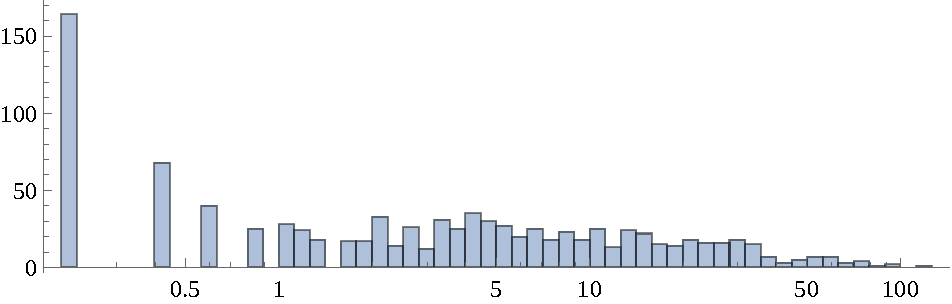
\includegraphics[width=0.75\textwidth,]{Figures/NA/Fig6.pdf}};
    \node[below=of img, node distance=1cm, yshift=1cm] {Daily Rainfall in Sydney};
    \node[left=of img, node distance=0cm, rotate=90, anchor=center,yshift=-0.7cm] {Count};
  \end{tikzpicture}
  \caption{Histogram of daily rainfall in Sydney, Australia, presented
    on a $\ln$ scale because the frequency of larger amounts of
    rainfall is significantly less. There is a peak in occurrence of
    the value $0$, which has a notable effect on the resulting model
    performance.}
  \label{fig:hist-weather}
\end{figure}

\begin{figure}
  \centering
  \begin{tikzpicture}
    \node (img)  {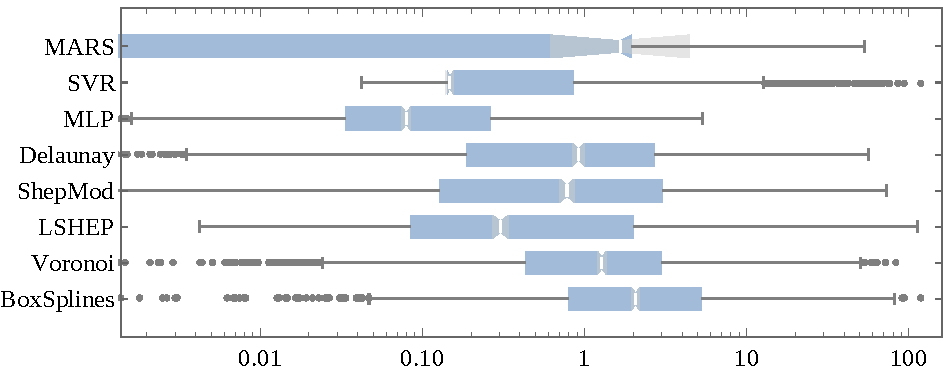
\includegraphics[width=0.8\textwidth,]{Figures/NA/Fig7.pdf}};
    \node[below=of img, node distance=1cm, yshift=1cm] {Sydney Rainfall Tomorrow Error};
  \end{tikzpicture}
  \caption{All models are applied to approximate the amount of
    rainfall expected on the next calendar day given various sources
    of local meteorological data, using $10$-fold cross validation.
    These boxes depict the median (middle bar), median $95\%$
    confidence interval (cones), quartiles (box edges), fences at
    $3/2$ interquartile range (whiskers), and outliers (dots) of
    absolute prediction error for each model. The errors are presented
    on a $\ln$ scale, mimicking the presentation in Figure
    \ref{fig:hist-weather}. The numerical data corresponding to this
    figure is provided in Table \ref{table:error-weather} in the
    Appendix.}
  \label{fig:error-weather}
\end{figure}

The third data set for the total daily rainfall in Sydney, Australia
\cite{williams2009rattle} provides a slightly higher dimensional
challenge for the interpolants and regressors. This data is composed
of many meteorological readings from the region in a day including:
min and max temperatures, sunshine, wind speed directions (converted
to coordinates on a circle), wind speeds, and humidities throughout
the day, day of the year (converted to coordinates on a circle), and
the model must predict the amount of rainfall tomorrow.

While Figure \ref{fig:hist-weather} makes MARS look far better than
other techniques, it only provides the best prediction for $11\%$ of
points. The MLP has the lowest absolute error for $56\%$ of points and
LSHEP is best for $28\%$. MARS likely achieves such a low first
quartile due to the high occurrence of the value zero in the data.
%% -------------------------------------------------------------------



%% -------------------------------------------------------------------
\subsection{Credit Card Transaction Amount ($n = 5562$, $d = 28$)}

\begin{figure}
  \centering
  \begin{tikzpicture}
    \node (img)  {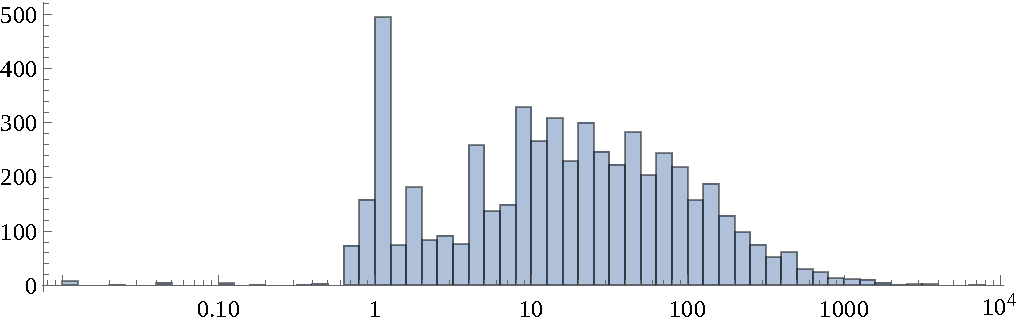
\includegraphics[width=0.75\textwidth,]{Figures/NA/Fig8.pdf}};
    \node[below=of img, node distance=1cm, yshift=1cm] {Credit Card Transaction Amount};
    \node[left=of img, node distance=0cm, rotate=90, anchor=center,yshift=-0.7cm] {Count};
  \end{tikzpicture}
  \caption{Histogram of credit card transaction amounts, presented on
    a $\ln$ scale. The data contains a notable frequency peak around
    $\$1$ transactions. Fewer large purchases are made, but some large
    purchases are in excess of five orders of magnitude greater than
    the smallest purchases.}
  \label{fig:hist-credit-card}
\end{figure}

\begin{figure}
  \centering
  \begin{tikzpicture}
    \node (img)  {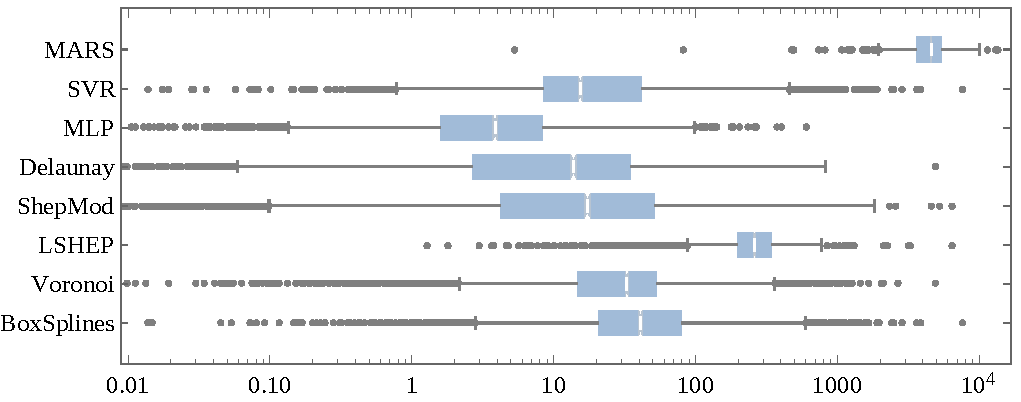
\includegraphics[width=0.8\textwidth,]{Figures/NA/Fig9.pdf}};
    \node[below=of img, node distance=1cm, yshift=1cm] {Transaction Amount Error};
  \end{tikzpicture}
  \caption{All models are applied to approximate the expected
    transaction amount given transformed (and obfuscated) vendor and
    customer-descriptive features, using $10$-fold cross validation.
    These boxes depict the median (middle bar), median $95\%$
    confidence interval (cones), quartiles (box edges), fences at
    $3/2$ interquartile range (whiskers), and outliers (dots) of
    absolute prediction error for each model. The absolute errors in
    transaction amount predictions are presented on a $\ln$ scale,
    just as in Figure \ref{fig:hist-credit-card}. The numerical data
    corresponding to this figure is provided in Table
    \ref{table:error-credit-card} in the Appendix.}
  \label{fig:error-credit-card}
\end{figure}

The fourth test data set, and the final with a real-valued range, is a
collection of credit card transactions
\cite{pozzolo2015calibrating}. The provided data carries no direct
real-world meaning, being the output of a principle component analysis
on the original hidden source data. This obfuscation is done to
protect the information of the credit card users. This data has the
largest dimension of all considered, at 28. A model for this data
predicts the transaction amount given the vector of principle
component information.

As can be seen in Figure \ref{fig:error-credit-card}, the MLP
outperforms all other algorithms at the first, second, third, and
fourth quartiles. The MLP produces the lowest absolute error
prediction for $80\%$ of transactions, Delaunay bests the remaining
$20\%$. It is likely that with less data, Delaunay would be the best
performer.
%% -------------------------------------------------------------------


%% -------------------------------------------------------------------
\subsection{High Performance Computing I/O ($n = 3016$, $d = 4$)}

\begin{figure}
  \centering
  \begin{tikzpicture}
    \node (img)  {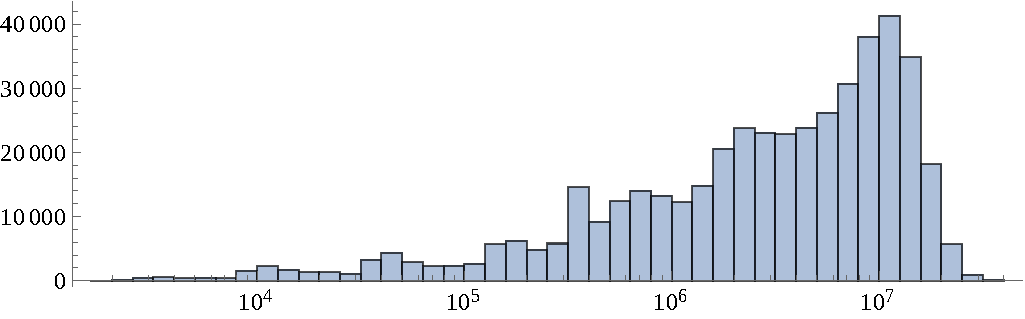
\includegraphics[width=0.75\textwidth,]{Figures/NA/Fig10.pdf}};
    \node[below=of img, node distance=1cm, yshift=1cm] {I/O Read Throughput};
    \node[left=of img, node distance=0cm, rotate=90, anchor=center,yshift=-0.7cm] {Count};
  \end{tikzpicture}
  \caption{Histogram of the raw throughput values recorded during all
    IOzone tests across all system configurations. The distribution is
    skewed right, with few tests having significantly higher
    throughput than most others. The data is presented on a $\ln$
    scale.}
  \label{fig:hist-throughput}
\end{figure}

\begin{figure}
  \centering
  \begin{tikzpicture}
    \node (img)  {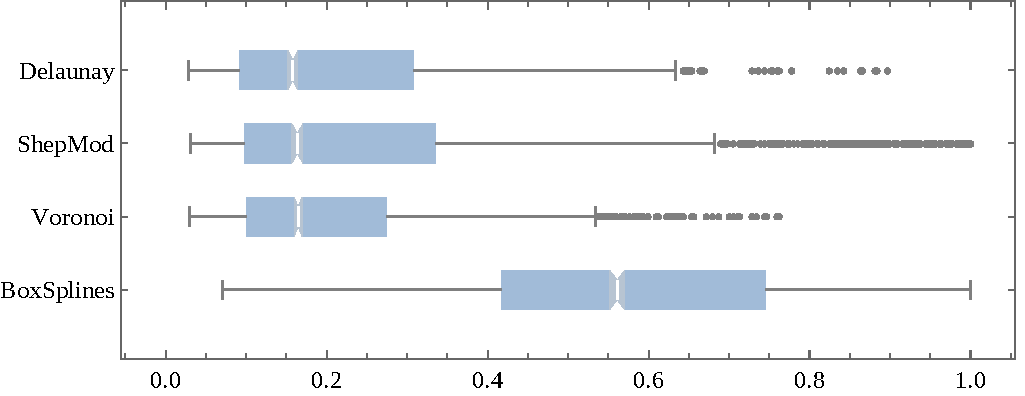
\includegraphics[width=0.8\textwidth,]{Figures/NA/Fig11.pdf}};
    \node[below=of img, node distance=1cm, yshift=1cm] {Read Throughput KS Statistic};
  \end{tikzpicture}
  \caption{The models directly capable of predicting distributions are
    applied to predicting the expected CDF of I/O throughput at a
    previously unseen system configuration, using $10$-fold cross
    validation. The KS statistic between the observed distribution at
    each system configuration and the predicted distribution is
    recorded and presented above. Note that the above figure is
    \textit{not} log-scaled like Figure \ref{fig:hist-throughput}. The
    numerical data corresponding to this figure is provided in Table
    \ref{table:error-throughput} in the Appendix.}
  \label{fig:error-throughput}
\end{figure}

The final of five data sets is derived from \cite{cameron2019moana},
which provides four-dimensional distribution data by executing the
IOzone benchmark \cite{iozone} on a computer system and varying the
system's file size, record size, thread count, and CPU frequency. At
each configuration, IOzone samples the I/O file-read throughput (in
bytes per second) 150 times. Empirical distribution function points
are computed from each set of 150 executions, which are interpolated
with a piecewise cubic Hermite interpolating polynomial
\cite{fritsch1980monotone} to approximate the CDF. All interpolation
algorithms with the exception of LSHEP are used to approximate these
CDFs from system configurations.

Delaunay achieves the lowest KS statistic for $62\%$ of
approximations, while Voronoi is best for the remaining $38\%$. Figure
\ref{fig:error-throughput} shows that while Delaunay may have more
best predictions, the behavior of Voronoi may be preferable.
%% -------------------------------------------------------------------


%% -------------------------------------------------------------------
\begin{figure}
  \centering
  \begin{tikzpicture}
    \node (img)  {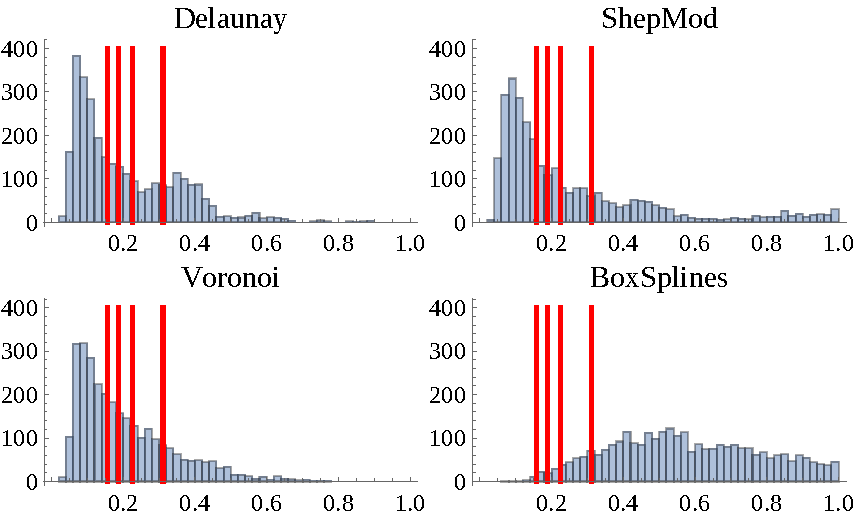
\includegraphics[width=0.8\textwidth]{Figures/NA/Fig12.pdf}};
    \node[below=of img, node distance=1cm, yshift=1cm] {KS Statistic for Predicted vs. Actual};
    \node[left=of img, node distance=0cm, rotate=90, anchor=center,yshift=-0.7cm] {Count of KS Statistic};
  \end{tikzpicture}
  \caption{Histograms of the prediction error for each interpolant
    that produces predictions as convex combinations of observed data,
    using $10$-fold cross validation. The histograms show the KS
    statistics for the predicted throughput distribution versus the
    actual throughput distribution. The four vertical lines represent
    cutoff KS statistics given $150$ samples for commonly used
    $p$-values 0.05, 0.01, 0.001, $10^{-6}$, respectively. All
    predictions to the right of a vertical line represent CDF
    predictions that are significantly different (by respective
    $p$-value) from the actual distribution according to the KS
    test. The numerical counterpart to this figure is presented in
    Table \ref{table:null-hypothesis-results}.}
  \label{fig:throughput-prediction}
\end{figure}

\begin{table}
  \renewcommand{\arraystretch}{1.3}
  \centering
  \begin{tabular}{c|c|c|c|c}
     & $p = .05$ & $p = .01$ & $p = .001$ & $p = 10^{-6}$\\
    \hline
    Delaunay & $\mathbf{50.3}\%$ & $\mathit{43.5}\%$ & $\mathit{36.2}\%$ & $\mathit{24.7}\%$\\
    ShepMod & $\mathit{51.4}\%$ & $44.8\%$ & $38.1\%$ & $27.7\%$\\
    Voronoi & $52.6\%$ & $\mathbf{43.4}\%$ & $\mathbf{34.4}\%$ & $\mathbf{19.1}\%$\\
    BoxSpline & $99.5\%$ & $98.5\%$ & $96.6\%$ & $89.5\%$\\
  \end{tabular}
  \caption{Numerical counterpart of the histogram data presented in
    Figure \ref{fig:throughput-prediction}. The columns display the
    percent of null hypothesis rejections by the KS-test when provided
    different selections of $p$-values for each algorithm. The
    algorithm with the lowest rejection rate at each $p$ is boldface,
    while the second lowest is italicized.}
  \label{table:null-hypothesis-results}
\end{table}


%% ===================================================================

Figure \ref{fig:throughput-prediction} expands on the KS statistic
results presented in Figure \ref{fig:error-throughput}. Agglomerate
errors for each algorithm resemble a Gamma distribution. The
percentages of significant prediction errors with varying $p$-values
are on display in Table \ref{table:null-hypothesis-results}. When
considering the $p=0.001$ results for each technique, a little over
one third of the predicted CDFs are significantly different from the
measured (and presumed) correct CDFs. However, it should be noted that
with 150 samples, the error of an empirical distribution function
(EDF) can reasonably be upwards of $.1$, which serves as a rough
estimate for the lower limit of achievable error. Globally, only a
third of Voronoi predictions fail to capture \textit{all} of the
characteristics of the CDFs at new system configurations.

\section{Discussion of Empirical Results}
                                                                      
\begin{table}
  \centering
  \begin{tabular}{c|r@{.}l|r@{.}l|r@{.}l}
    Algorithm & \multicolumn{2}{c|}{Avg. \% Best} & \multicolumn{2}{c|}{\multilinecell{Avg. Fit or \\ Prep. Time (s)}} & \multicolumn{2}{c}{Avg. App. Time (s)}\\
    \hline
    MARS & \quad\quad$4$&$6$ & \,\quad$20$&$0$ & \quad\quad$0$&$001$\\
    SVR & $\mathit{21}$&$\mathit{1}$ & $\mathbf{0}$&$\mathbf{5}$ & $\mathbf{0}$&$\mathbf{0001}$\\
    MLP & $\mathbf{42}$&$\mathbf{1}$ & $200$&$0$ & $0$&$001$\\
    Delaunay & $6$&$0$ & $1$&$0$ & $1$&$0$\\
    ShepMod & $18$&$4$ & $\mathit{0}$&$\mathit{7}$ & $\mathbf{0}$&$\mathbf{0001}$\\
    LSHEP & $8$&$4$ & $2$&$0$ & $\mathbf{0}$&$\mathbf{0001}$\\
    Voronoi & $0$&$5$ & $1$&$0$ & $0$&$04$\\
    BoxSpline & $0$&$2$ & $0$&$8$ & $\mathit{0}$&$\mathit{0005}$\\
  \end{tabular}
  \caption{This average of Appendix Tables
    \ref{table:best-forest-fire}, \ref{table:best-parkinsons},
    \ref{table:best-weather}, and \ref{table:best-credit-card}
    provides a gross summary of overall results. The columns display
    (weighted equally by data set, \textit{not} points) the average
    frequency with which any algorithm provided the lowest absolute
    error approximation, the average time to fit/prepare, and the
    average time required to approximate one point. The times have
    been rounded to one significant digit, as reasonably large
    fluctuations may be observed due to implementation hardware.
    Interpolants provide the lowest error approximation for nearly one
    third of all data, while regressors occupy the other two
    thirds. This result is obtained without any customized tuning or
    preprocessing to maximize the performance of any given
    algorithm. In practice, tuning and preprocessing may have large
    effects on approximation performance.}
  \label{table:avg-performance}
\end{table}

Table \ref{table:avg-performance} summarizes results across the four
test data sets with real-valued ranges. The interpolants discussed in
this chapter produce the \textit{best} approximations roughly one third
of the time, and produce competitive approximations for almost all
data sets. These test problems are almost certainly
\textit{stochastic} in nature, but the high dimension leads to greater
data sparsity and model construction cost, making interpolation more
competitive.

The major advantages to interpolation lie in the near absence of
\textit{fit} time. Delaunay, LSHEP, and ShepMod all require pairwise
distance calculations, for numerical robustness (Delaunay) and to
determine the radii of influence for data points (LSHEP and
ShepMod). At least hundreds, and sometimes hundreds of thousands of
predictions can be made by the interpolants before the most widely
used regressor (MLP) finishes fitting these relatively small data
sets.  However, the computational complexities of all interpolants
presented are greater than linear in either dimension or number of
points, whereas the regressors' nonlinear complexity in dimension
generally comes from the model fitting optimization.

The theoretical results presented in this chapter directly apply to
Delaunay interpolation, however the performance of Delaunay does not
appear significantly better than other algorithms on these data sets.
This observation may be due to the stochastic nature of the data, but
it also speaks to the power of the approximations generated by the
different interpolation methods.  The strong performance of other
interpolants suggests that theoretical results similar to those
presented in this work can be achieved for the other interpolants
under reasonable assumptions.

Finally, most of the interpolants presented in this work benefit from
the ability to model any function over real $d$-tuples with a range
that is closed under convex combinations. The results of the
distribution prediction case study indicate that interpolants can
effectively predict CDFs. The error analysis for that work relies on
the KS statistic, which captures the worst part of any prediction and
hence provides a conservatively large estimate of approximation
error. The average absolute errors in the predicted CDFs are always
lower than the KS statistics. However, the KS statistic was chosen as
a metric because of the important surrounding statistical theory. A
nonnegligible volume of predictions provide impressively low levels of
average absolute error in that final case study.

\section{Takeaway from Empirical Tests}

The major contributions of this work are: 1) new uniform theoretical
error bounds for piecewise linear interpolation in arbitrary
dimension; 2) an empirical evaluation across real-world problems that
demonstrates interpolants produce competitively accurate models of
multivariate phenomenon when compared with common regressors for
sparse, moderately high dimensional problems (Section
\ref{sec:error_data}); and 3) a demonstration that some interpolants
generalize to interpolation in function spaces, preserving
monotonicity (with CDFs, e.g.), neither of which common regressors can
do.

The various interpolants discussed in this work have been
demonstrated to effectively approximate multivariate phenomena up to
$30$ dimensions. The underlying constructions are theoretically
straightforward, interpretable, and yield reasonably accurate
predictions. Most of the interpolants' computational complexities make
them particularly suitable for applications in even higher
dimension. The major benefits of interpolation are seen when only a
small number of approximations ($\leq 1000$) are made from data and
when there are relatively few data points for the dimension (for
empirical results presented, $\log_d n \leq 5$). These findings
encourage broader application of interpolants to multivariate
approximation in science
